\documentclass[a4paper]{article}

\usepackage{xparse}
\usepackage{colortbl}
\usepackage{circuitikz}
\usepackage{cancel}
\usepackage{siunitx}
\usepackage{multirow}
\usepackage{array}
\usepackage[table, xcdraw, dvipsnames]{xcolor}
\usepackage{times}
\usepackage{tikz}
\usepackage[top=1.5cm, bottom=1.5cm, left=2.5cm, right=1.5cm]{geometry}
\usepackage{graphicx}
\usepackage{anyfontsize}
\usepackage{fancyhdr}
\usepackage{indentfirst}
\usepackage{amsmath}
\usepackage[spanish, es-tabla]{babel}
\usepackage[utf8]{inputenc}
\usepackage[explicit]{titlesec}
\usepackage{etoolbox}
\usepackage{multicol}
\usepackage{enumitem}
\usepackage[labelformat=simple, labelsep=none]{caption}
\usepackage{booktabs}
\usepackage{amsfonts}
\usepackage[version=4]{mhchem}
\usepackage{float}
\usepackage{lastpage}
\usepackage{subcaption}
\usepackage{hyperref}
\usepackage{capt-of}

\setkeys{Gin}{keepaspectratio}

\definecolor{gold}{RGB}{212,175,55}
\definecolor{silver}{RGB}{192,192,192}
\definecolor{gold}{rgb}{1.0, 0.84, 0.0}
\newcommand{\diodoSilicio}[1]{
    \begin{minipage}{2cm}
        \begin{center}
            \begin{circuitikz}[scale=0.5]
                \draw[line width=1pt] (-2,0) -- (-1,0);
                \draw[line width=1pt] (2,0) -- (1,0);

                \filldraw[fill=black!75, draw=black] (-1, -0.5) rectangle (1, 0.5);

                \fill[gray!60] (0.6, -0.5) rectangle (0.8, 0.5);

                \node at (0, -1) {\texttt{#1}};
            \end{circuitikz}
        \end{center}
    \end{minipage}
}
\newcommand{\diodoGermanio}[1]{
    \begin{minipage}{2cm} 
        \begin{center}
            \begin{circuitikz}[scale=0.5]
                \draw[line width=0.8pt] (-2.5,0) -- (-1.5,0);
                \draw[line width=0.8pt] (2.5,0) -- (1.5,0);

                \filldraw[fill=white, draw=black] (-1.5, -0.4) rectangle (1.5, 0.4);
                \fill[orange!80] (-1.5, -0.25) rectangle (1.5, 0.25);
                \fill[gray!95] (1.2, -0.4) rectangle (1.5, 0.4);
                \node at (0, -0.9) {\texttt{#1}};
            \end{circuitikz}
        \end{center}
    \end{minipage}
}

\newcommand{\resistencia}[4]{
    \begin{minipage}{2cm}
        \begin{center}
            \begin{tikzpicture}
                \draw(-0.4cm, -0.15cm) rectangle (0.4cm, 0.15cm);
                \fill[resistor] (-0.4cm, 0) -- (-0.5cm, 0);
                \draw (-0.4cm, 0) -- (-0.5cm, 0);
                \draw (0.4cm, 0) -- (0.5cm, 0);
                \fill[#1] (-0.35cm, -0.15cm) rectangle (-0.25cm, 0.15cm);
                \fill[#2] (-0.15cm, -0.15cm) rectangle (-0.05cm, 0.15cm);
                \fill[#3] (0.05cm, -0.15cm) rectangle (0.15cm, 0.15cm);
                \fill[#4] (0.25cm, -0.15cm) rectangle (0.35cm, 0.15cm);
            \end{tikzpicture}
        \end{center}
    \end{minipage}
}


\NewDocumentCommand{\resaltar}{ O{yellow} m }{%
  \begingroup
  \setlength{\fboxsep}{1pt} %Padding
  \colorbox{#1}{\strut\ensuremath{#2}}%
  \endgroup
}

\renewcommand{\theenumi}{\Roman{enumi}}

\newcommand{\recuadrar}[2]{
    \begin{center}
        \begin{tabular}{m{#1}}
            \toprule
            \multicolumn{1}{|c|}{\hspace{5pt}#2\hspace{5pt}} \\
            \bottomrule
        \end{tabular}
    \end{center}
}

\newcommand{\ecuacion}[1]{
    \begin{center}
        $#1$
    \end{center}
}

\newcommand{\longsection}[2]{%
    \section[#1]{\parbox{\columnwidth}{#1}}
}

\newcommand{\saltoPag}[0]{%
    \newpage\noindent\thispagestyle{fancy}%
    \begin{tikzpicture}[remember picture, overlay]
        \draw[line width=0.4pt, color=gray!50] (8.5cm, -0.4cm) -- (8.5cm, -26cm);
    \end{tikzpicture}%
    \ignorespaces{}
}

\newcommand{\midTitle}[2]{%
    \begin{center}
        \textcolor{#1}{\underline{#2}} 
    \end{center}
}


\newcommand{\sangria}[0]{\par\noindent\hspace*{15pt}}

\newcommand{\longsubsection}[2]{%
    \subsection[#1]{\parbox{\columnwidth}{#1}}%
}
\captionsetup{
    format=hang,
    labelfont={bf},
    textfont=normalfont,
    labelsep=colon,
    justification=centering,
    singlelinecheck=true
}

\newcommand{\imagen}[3][]{
    \vspace{5pt}
    \begin{center}
        \begin{tikzpicture}
            \node[inner sep=2pt] (image) {\includegraphics[width=#2]{#3}};
            \draw[line width=1pt, color={rgb:red,251;green,73;blue,52}] (image.south west) rectangle (image.north east);
        \end{tikzpicture}
        \ifx\\#1\\
            \captionof{figure}{}
        \else
            \captionof{figure}{#1}
        \fi 
        \label{fig:#2}
    \end{center}
    \vspace{5pt}
}



\begin{document}
    \author{}\date{}\title{}
\thispagestyle{empty}
\begin{tikzpicture}[remember picture, overlay]
    \pgftransformshift{\pgfpoint{0cm}{0cm}}
    \draw [line width=2pt](1cm,-1cm) -- (1cm,-27.7cm) -- (14cm, -27.7cm) -- (14cm, -1cm) -- (1cm, -1cm);
    \draw[line width=2pt] (15cm, -27.7cm) -- (19cm,-27.7cm) -- (19cm, -1cm) -- (15cm, -1cm) --  (15cm, -27.7cm);
    \node [line width=2pt] at (17cm, -3.5cm) {
\includegraphics[width=3cm]{./imagenes/utn.png}};
	\node [line width=2pt] at (7.5cm, -9cm) {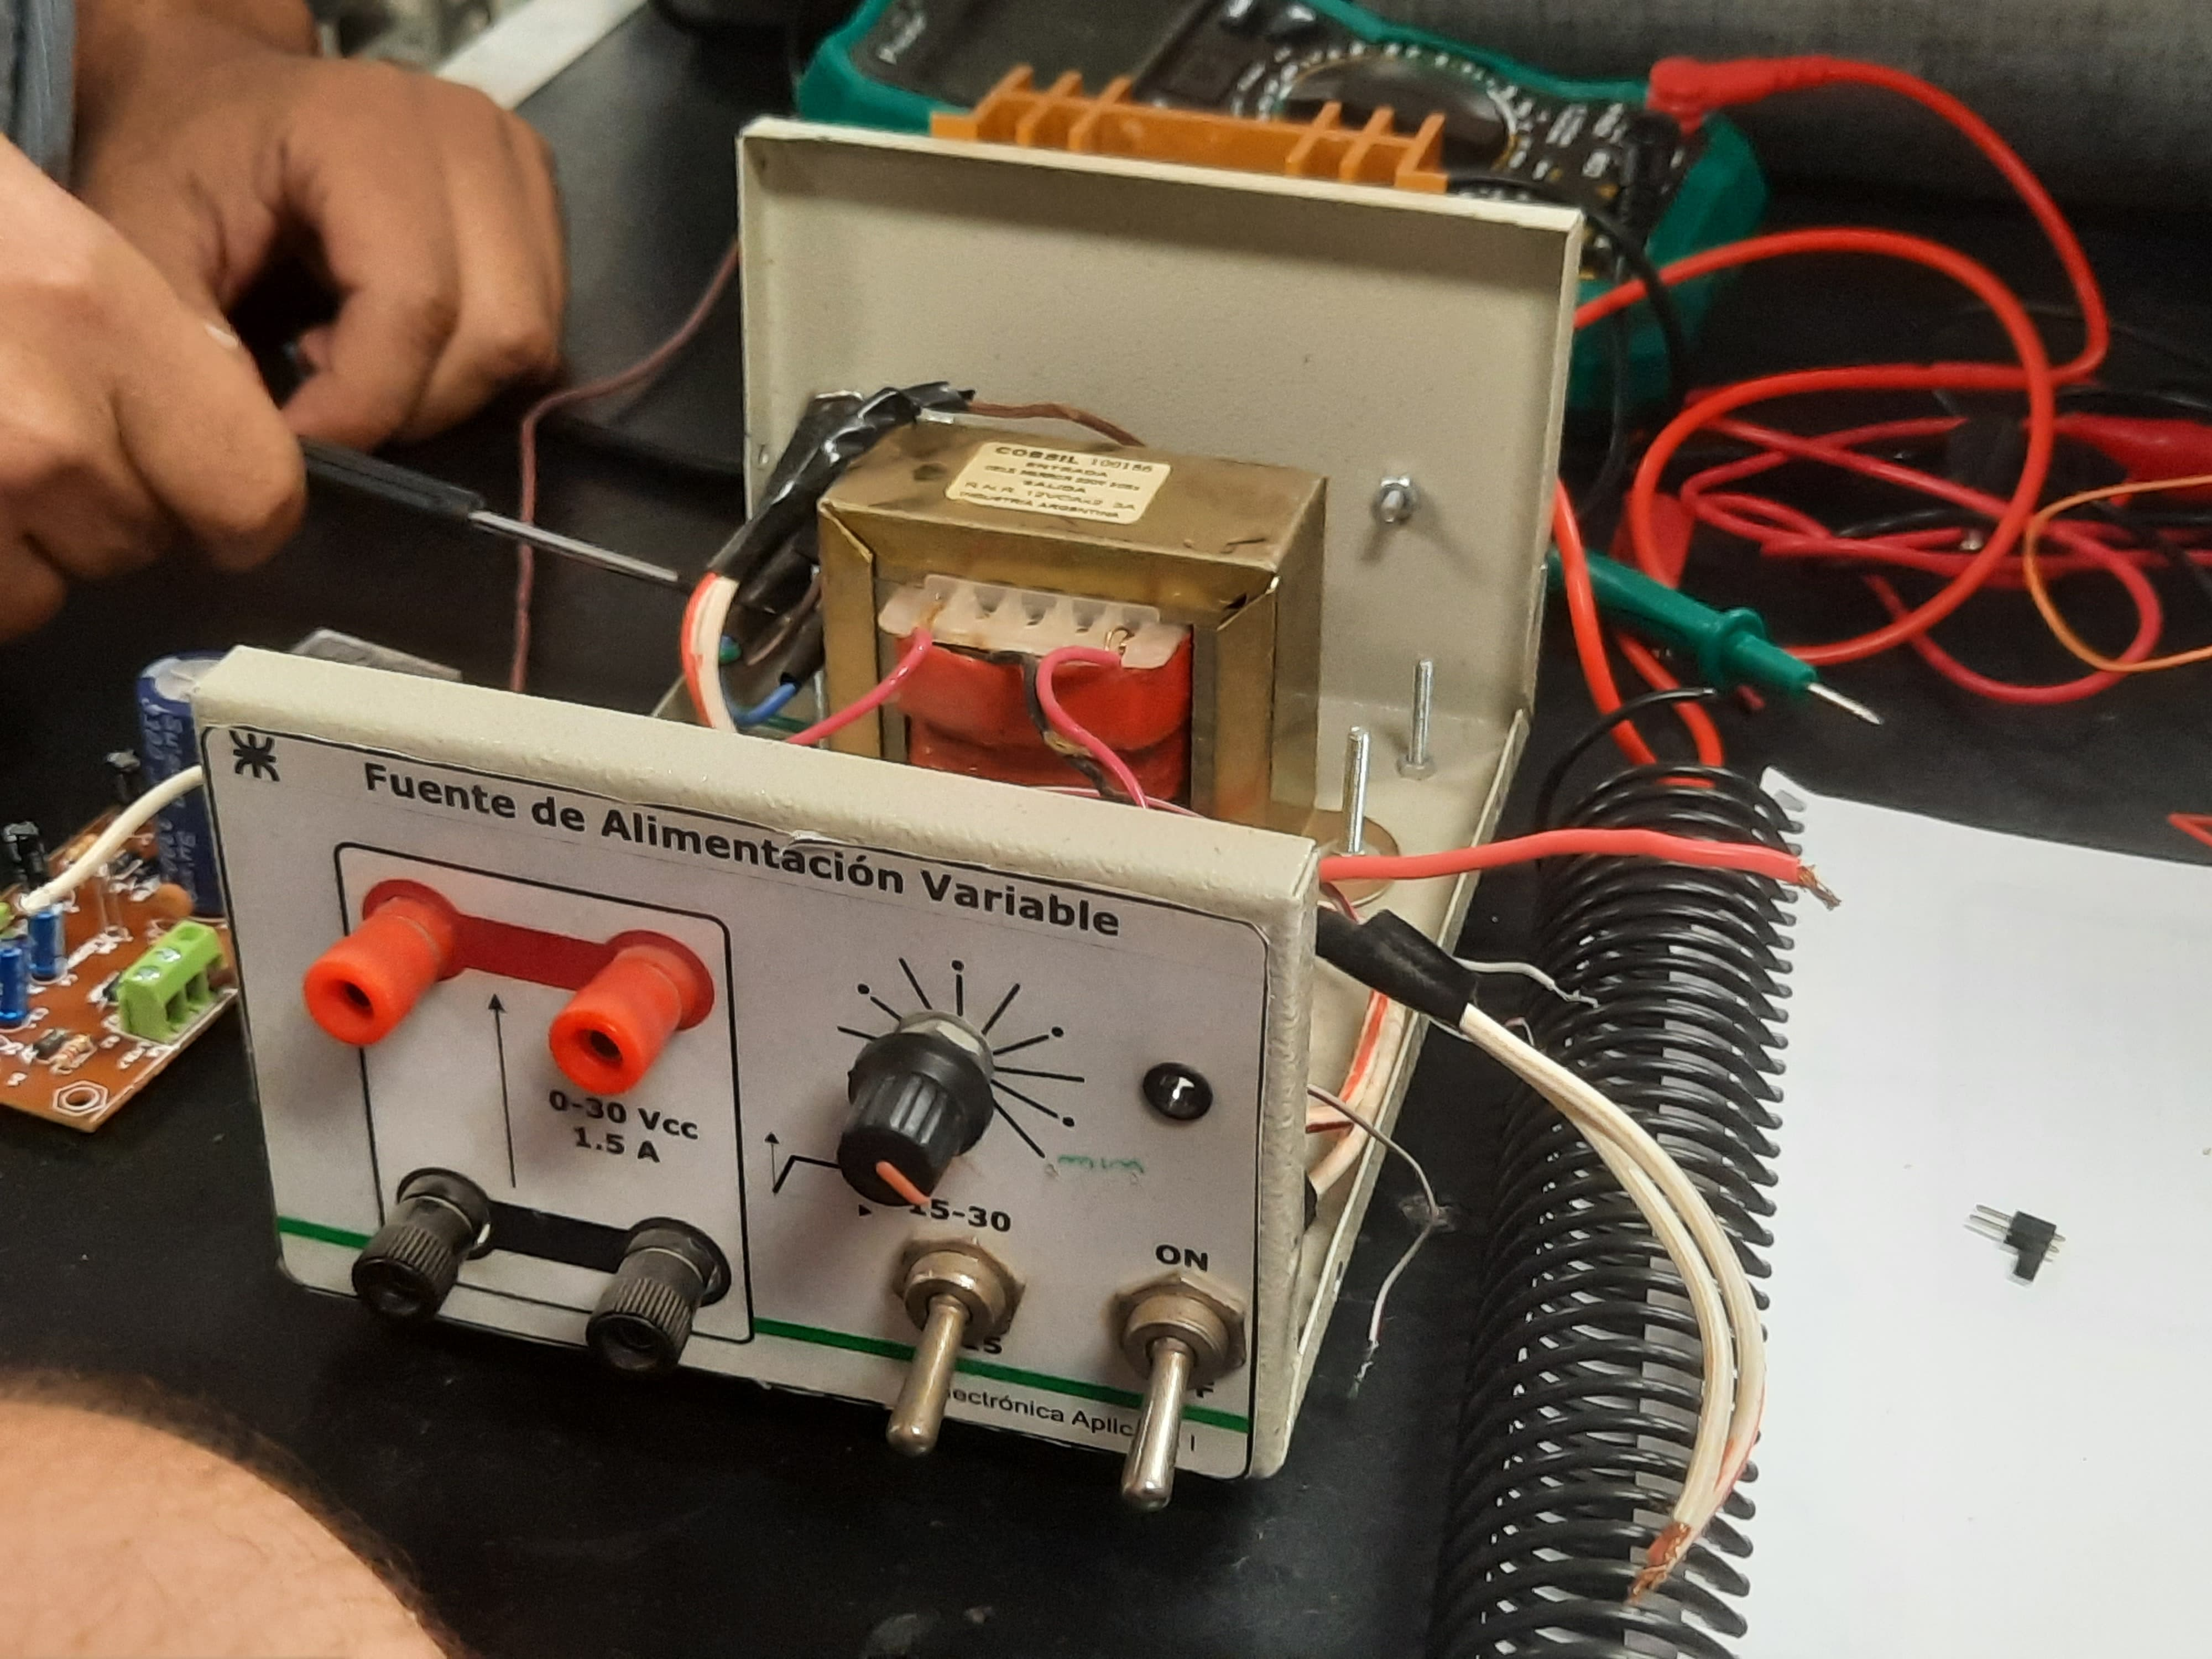
\includegraphics[width=8cm]{./imagenes/portada.jpg}};
    \node at (17cm, -7cm) {\scalebox{5}{\textbf{U}}};
    \node at (17cm, -9cm) {\scalebox{5}{\textbf{T}}};
    \node at (17cm, -11cm) {\scalebox{5}{\textbf{N}}};
    \node at (17cm, -14cm) {\scalebox{5}{\textbf{F}}};
    \node at (17cm, -16cm) {\scalebox{5}{\textbf{R}}};
    \node at (17cm, -18cm) {\scalebox{5}{\textbf{C}}};
    \node at (7.5cm, -14cm) {\scalebox{3}{\textbf{Ensayos fuente}}};
    \node at (7.5cm, -15cm) {\scalebox{3}{\textbf{de}}};
    \node at (7.5cm, -16cm) {\scalebox{3}{\textbf{alimentación}}}; 
    \node at (7.5cm, -23.5cm) {
	\begin{minipage}[c]{12cm}
	    \begin{itemize}
            \raggedright
            \item \fontsize{12}{12}\selectfont \textbf{Autores:} 
                \begin{itemize} \item Manuel León Parfait - Leg. 406599  \item Marcos Raúl Gatica - Leg. 402006  \item Valentino Rao - Leg. 402308  \end{itemize}
            \item \fontsize{12}{12}\selectfont \textbf{Curso:} 3R1  \\
            \item \fontsize{12}{12}\selectfont \textbf{Asignatura:} Electrónica Aplicada.
            \item \fontsize{12}{12}\selectfont \textbf{Institución:} Universidad Tecnológica Nacional - Facultad Regional de Córdoba.
        \end{itemize}
    \end{minipage}};
\end{tikzpicture}

    \renewcommand{\normalsize}{\fontsize{12}{18}\selectfont}
\newgeometry{left=2.5cm, right=1.5cm, top=1.5cm, bottom=1.5cm}
\fancyhf{}
\renewcommand{\headrulewidth}{0pt}
\renewcommand{\footrulewidth}{0.4pt}
\fancyfoot[R]{[Parfait M. - Rao V. - Gatica M.] [\textbf{pág.\ \thepage} de \pageref{LastPage}]}
\setlength{\footskip}{0.5cm}
\titleformat{\section}[hang]{\fontsize{12}{12}\bfseries}{\thesection.}{0.5em}{\underline{#1}}
\setlength{\columnsep}{10mm}
\raggedcolumns
\renewcommand{\bottomfraction}{0.5}
\widowpenalty=10000
\clubpenalty=10000
\enlargethispage{-1cm}

    \newpage\thispagestyle{empty}\text{}\newpage\newpage\thispagestyle{empty}\setcounter{page}{0}\tableofcontents\newpage\newpage\thispagestyle{empty}\text{}\setcounter{page}{0}

    \saltoPag{}

    \begin{multicols}{2}
        \setlength{\columnsep}{10mm}
        \section{Planteamiento e introducción teórica} 
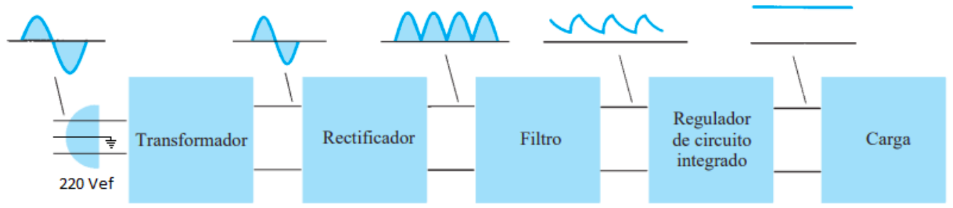
\includegraphics[width=7.8cm]{./imagenes/Diagra.png}
\subsection{Transformador}
\sangria{} El transformador tiene dos funciones:

\begin{itemize}
    \item Aislar galvánicamente de la línea de 220 V 50 Hz a la fuente, ya que
    primario y secundario están acoplados magnéticamente.
    \item Reducir la tensión de 220 V a 12/24 V o el valor que sea necesario según
    las necesidad de la fuente a construir.
\end{itemize}

\sangria{} El trasnformador  utilizado en esta funte es un 12+12 X 3A y su simbolo es el siguiente:

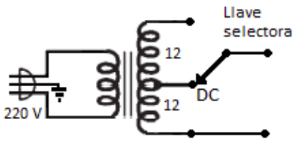
\includegraphics[width=6cm]{./imagenes/transfo.png}

\sangria{} La entrada del transformador es la tensión alterna de 220 V y la salida es la tensión alterna de 12V+12V. La corriente alterna se conecta a la entrada del trasnformador a un inductor que produce un campo magnético que mediante inducción electromagnética produce una corriente alterna en el secundario que deende del bobinado de los inductores. 
\sangria{} Se especifica que al transformador se le pueden extaer hasta 3A, lo que significa que en la rectificación de onda completa con punto medio se extrae 1,5A por rama 

\subsection{Rectificador}
\sangria{} La función del rectificador es convertir la tensión alterna en una continua pulsante, esto lo lleva a cabo un puente de diodos que permite el paso de la corriente en un sentido y bloquea el paso en el otro. 
\begin{center}
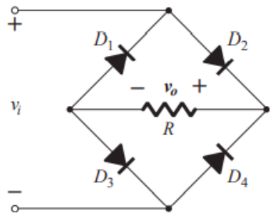
\includegraphics[width=6cm]{./imagenes/puent.png}
\end{center}
\sangria{} Esto ocurre ya que los diodos Conducen corriente en un solo sentido y al conectarlos en inversa, extremo positivo al negativo, no permiten el paso de la corriente.

\columnbreak

\sangria{} Al entrar una tensión alterna al puente como la de la siguiente figura: 
\begin{center}
    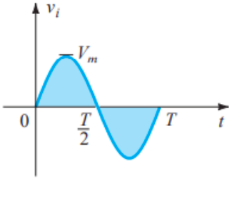
\includegraphics[width=6cm]{./imagenes/Alte.png}
\end{center}

\sangria{} Para el semiciclo positivo conducen D2 y D3 a través de la carga R:
\begin{center}
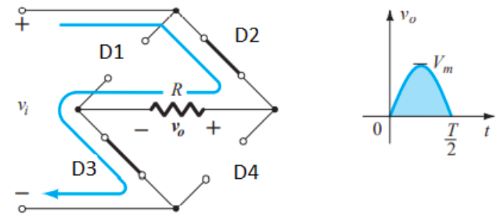
\includegraphics[width=6cm]{./imagenes/semic.png}
\end{center}
\sangria{} Y para el semiciclo negativo conducen D1 y D4 a través de la carga R cambiando el sentido de la onda y eliminando el semiciclo negativo:
\begin{center}
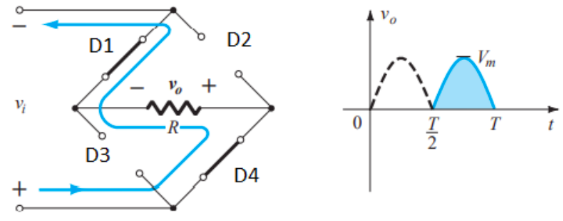
\includegraphics[width=6cm]{./imagenes/semisic2.png}
\end{center}

\paragraph{} Tensión a la salida del rectificador:

\begin{center}
    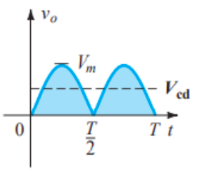
\includegraphics[width=6cm]{./imagenes/puentesal.png}
\end{center}

\begin{itemize}
    \item $V_{cd}$: Es el valor medio de voltaje que se obtendría midiendo con un multímetro en voltaje de corriente continua.
    \item $V_{m}$: Valor pico.
    \item La frecuencia de la onda pulsante es el doble de la señal de entrada, 100Hz.
\end{itemize}

\saltoPag{}

\sangria{} El voltaje pico inverso (VPI) es el voltaje máximo que pasara por el diodo en polarización inversa. 

\begin{center}
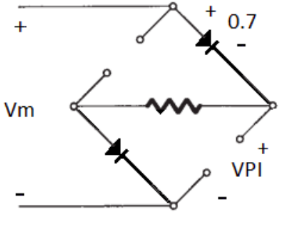
\includegraphics[width=5cm]{./imagenes/VPI.png}
\end{center}

\sangria{} Aplicando la ley de Kirchoff de voltaje en la malla externa:
\begin{equation*}
    V_m - 0,7 - VPI = 0 \Rightarrow VPI = V_m - 0,7
\end{equation*}

\sangria{} \textbf{Especificaciones de los diodos:} 
\sangria{} La corriente máxima que entrega el transofrmador es de 1.5, 0.75A en cada diodo. Pero el regulador LM317 es de 1.5A pero puede suministrar durante un
periodo corto de tiempo hasta 2.1 A, luego actúa la protección de sobrecorriente, lo que hace que superemos por un pequeño margen el limite de corriente de los diodos.
Como no se fabrican diodos de 2A se utilizan de 3A.

\subsection{Filtrado}
La onda pulsante a la salida del rectificador no es apta para alimentar
equipos electrónicos por ello se le agrega un capacitor que se carga y se descarga actunado como filtro para alizarla, la formula para calcular el mismo es:

\begin{equation*}
    C = \frac{I_L}{2 \cdot f_{salida} \cdot \Delta V}
\end{equation*}
\begin{itemize}
    \item $I_L$: Corriente de carga.
    \item $f_{salida}$: Frecuencia de la onda de salida del rectificador.
    \item $\Delta V$: Voltaje pico a pico del riple.
    \item $C$: Valor del capacitor
\end{itemize}

\sangria{} \textbf{Corriente Pico en los diodos:}
\sangria{} Si aumentamos la capacidad del filtro disminuye la amplitud del riple y
aumenta el voltaje promedio, pero esto afecta la corriente pico de los
diodos como se puede observar en la grafica.

\begin{center}
    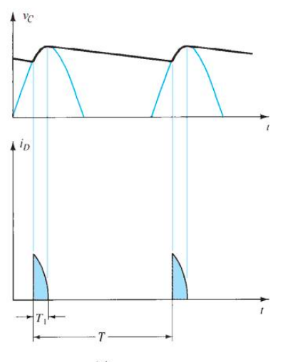
\includegraphics[width=5cm]{./imagenes/Dyc.png}
    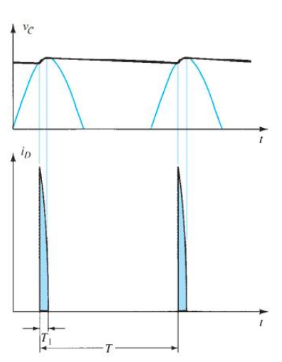
\includegraphics[width=5cm]{./imagenes/Dyc1.png}
\end{center}

\subsection{Regulador}
\sangria{} La función del regulador de tensión es mantener constante la tensión de
salida a pesar de las fluctuaciones de la corriente en la carga y de la
tensión de línea.
\sangria{} Por otra parte atenúa el riple en el orden de unas 1000 veces, por ejemplo
si tenemos 3V de riple a la entrada del regulador a la salida quedaran 3mV.

\begin{center}
    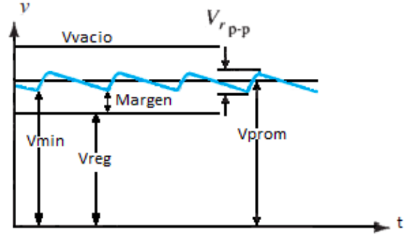
\includegraphics[width=5cm]{./imagenes/rplrg.png}
\end{center}

\begin{itemize}
    \item $\delta =V_{r_{p-p}}$: Voltaje pico a pico del riple.
    \item $V_{prom}$: Voltaje promedio.
    \item $V_{min}$: Voltaje mínimo.
    \item $V_{reg}$: Voltaje regulado.
    \item Margen: 3V para LM317.
\end{itemize}

\saltoPag{}

\paragraph{} Conexiones del regulador LM317(1.2 A 37V):
\vspace{0.5cm}
\begin{center}
    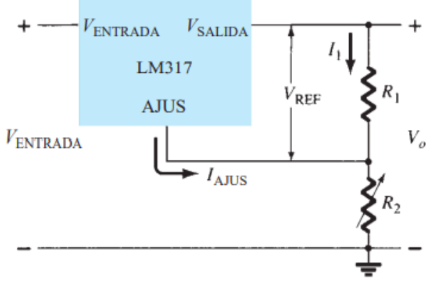
\includegraphics[width=6cm]{./imagenes/Diagrama317.png}
\end{center}

\sangria{} Algunas espidificaciones de la oja de datos:


\begin{itemize}
    \item $V_{REF}=1.25V$
    \item $\theta_{JC} = 3 W/ ^\circ\mathrm{C} $
    \item $I_{AJUS} = 50\mu A$
    \item $V_{diferencial-m \tilde{a} xima}=\\V_{ENTRADA}-V_{SALIDA}=40V$
    \item $T_{Juntura-m\tilde{a}xima}=125 ^\circ\mathrm{C}$
    \item $I_1=I_{REF}=\frac{V_{REF}}{R_1}$
    \item $I_{max}=1.5A$
    \item LM317 encapsulado TO-220 disipa 15W y encapsulado TO-3 20W.
\end{itemize}

\begin{center}
\textbf{Protecciones internas del LM317:}
\end{center}
\sangria{} \textbf{Protección de sobrecorriente:} significa que si se supera el limite permisible de corriente de salida actúa la protección interna evitando el daño del mismo.

\sangria{} \textbf{Protección de sobre temperatura:} si las dimensiones del disipador no son acordes para evacuar el calor que se genera debido a la disipación de potencia, se eleva la temperatura de la juntura sobrepasando el límite permisible
actuando la protección interna.

\sangria{} \textbf{Área de operación segura de potencia del transistor de salida:} si
bien no se puede estar excediendo el límite de corriente, puede ser que la
magnitud del voltaje entre la entrada y la salida haga que se supere la potencia máxima permisible que puede disipar el regulador. Por lo que actúa la protección interna.

\sangria{} Exepto en el regulador de funcionamiento, ni bien cesa la condición
indeseable el regulador restablece su funcionamiento.

\columnbreak
\text{}
        \section{Punto 2: Mediciones y Ensayos}
    \subsection{Elementos utilizados}
    
    \begin{itemize}
        \item Reostato de 50$\Omega$.
        \item Pinza amperométrica.
        \item Multímetro.
        \item Osciloscopio.
    \end{itemize}

    \indent{Para realizar las mediciones se utilizó un reostato de 50$\Omega$ que simula la carga del sistema y una pinza amperométrica para medir la corriente. También se utilizó un multímetro para medir la tensión y temperatura del LM317, finalmente se utilizó un osciloscopio para visualizar la señal filtrada.}

    \subsection{Mediciones punto alto y punto bajo sin LM317}

    \indent{El objetico de esta parte es medir el RV (regulación de voltage), el FR (factor de ripple) y la resistencia interna antes de pasar por el circuito del LM317, las escuaciones para calcular estos valores son las siguientes:}

    \begin{equation}
        RV = \frac{V_{\text{vacío}}-V_{\text{carga maxima}}}{V_{\text{carga maxima}}} \cdot 100\%
    \end{equation}

    \begin{equation}
        FR = \frac{V_{\text{ripple}}}{V_{\text{carga maxima}}} * 100\%
    \end{equation}

    \begin{equation}
        R_{int} = \frac{V_{\text{vacío}} - V_{\text{carga maxima}}}{I_{\text{carga}}}
    \end{equation}

    \begin{equation}
        V_{\text{ripple}} = \frac{V_{\text{ripple}}*0,5}{\sqrt{2}}
    \end{equation}

    \saltoPag{}

    \subsection{Punto bajo de la fuente}

    \indent{Para el punto bajo de la fuente medimos la tensión en el circuito desde cuando no tiene carga (en el vacio), hasta una carga de $1,5 A$, esto corresponde a la llave selectora que entrega desde $0 - 15 V$ de tensión.}

    \begin{itemize}
        \item Tensión en vacío: $V_{\text{vacío}} = 17,56 V$.
        \item Tensión con $0,50 A$: $V_{\text{carga}} = 15,20 V$.
        \item Tensión con $0,75 A$: $V_{\text{carga}} = 14,60 V$.
        \item Tensión con $1,00 A$: $V_{\text{carga}} = 14,04 V$.
        \item Tensión con $1,25 A$: $V_{\text{carga}} = 13,53 V$.
        \item Tensión con $1,50 A$: $V_{\text{carga maxima}} = 13,11 V$.
        \item Tensión de ripple Multimetro True RMS: $V_{\text{ripple}} = 0,89 V$. 
        \item Tensión de ripple Osciloscopio: $V_{\text{ripple}} = 0,919 V$.
    \end{itemize}

    \midTitle{black}{Resultados del Punto Bajo de la Fuente}
    
    \begin{itemize}
        \item $RV = \frac{17,56 - 13,11}{13,11} * 100\% = 33\%$.
        \item $FR = \frac{0,89}{13,11} * 100\% = 6,81\%$.
        \item $R_{int} = \frac{17,56 - 13,11}{1,50} = 2,96 \Omega$.
    \end{itemize}

    \subsection{Punto alto de la fuente}
    
    \indent{Para el punto alto de la fuente medimos la tensión en el circuito desde cuando no tiene carga (en el vacio), hasta una carga de $1,5 A$, esto corresponde a la llave selectora que entrega desde $15 - 30 V$ de tensión.}

    \begin{itemize}
        \item Tensión en vacío: $V_{\text{vacío}} = 35,52 V$.
        \item Tensión con $0,50 A$: $V_{\text{carga}} = 30,59 V$.
        \item Tensión con $0,75 A$: $V_{\text{carga}} = 29,61 V$.
        \item Tensión con $1,00 A$: $V_{\text{carga}} = 28,28 V$.
        \item Tensión con $1,25 A$: $V_{\text{carga}} = 26,93 V$.
        \item Tensión con $1,50 A$: $V_{\text{carga maxima}} = 25,75 V$.
        \item Tensión de ripple Multimetro True RMS: $V_{\text{ripple}} = 0,85 V$.
        \item Tensión de ripple Osciloscopio: $V_{\text{ripple}} = 0,84 V$.
    \end{itemize}

    \midTitle{black}{Resultados del Punto Alto de la Fuente}
    \begin{itemize}
        \item $RV = \frac{35,52 - 25,75}{25,75} = 0,3794 = 37,94\%$.
        \item $FR = \frac{0,85}{25,75} * 100\% = 3,30\%$.
        \item $R_{int} = \frac{35,52 - 25,75}{1,50} = 6,51 \Omega$.
    \end{itemize}

    \subsection{Regulación LM317 (Punto Alto)}

    \indent{En esta parte de los ensayos se busca medir la regulación del LM317 con una carga de $1,5 A$, como el LM317 trabaja en condiciones de maxima  potencia, midiendo su temperatura y calculando la temperatura de la juntura y si nuestra fuente regula correctamente.}

 \begin{center}
    \begin{tabular}{ c|c|c }
        & Mínimo & Máximo \\
        \midrule
        Punto Bajo & 0,31 & 15,31 \\
        Punto Alto & 0,41 & 30,46 \\
    \end{tabular}
\end{center}

    \begin{itemize}
        \item Tensión en el vacío: $V_{\text{vacío}} = 15,74 V$.
        \item Tensión con $1,50 A$: $V_{\text{carga maxima}} = 15,60s V$.
        \item Tensión de ripple osciloscopio: $V_{\text{ripple}} =  1,414 * 10^{-3} V$.
    \end{itemize}

    \midTitle{black}{Resultados del LM317 (Punto Alto)}
    \begin{itemize}
        \item $RV = \frac{15,74 - 15,60}{15,60} * 100\% = 0,89743 = 8,97\%$.
        \item $FR = \frac{1,414 * 10^{-3}}{15,60} * 100\% = 9,065 * 10^{-3}\%$.
    \end{itemize}

    
    \indent{Ecuación para calcular la temperatura de la juntura del LM317}
    %\vspace{-0.2cm}
    \begin{equation}
        T_{J} = T_{C} +P_{D} * \theta_{JC}
    \end{equation}

    \indent{En estas condiciones el LM317 esta disipando la máxima potencia $14.98 W$, ya que lo hicimos trabajar con una carga de $1,42 A$ y una tensión de $10,33 V$, el valor de $\theta_{JC}$ es de $3 \frac{C}{W}$, y la temperatura del encapsulado del LM317 medida fue  de $T_{C} = 70 C$.}

    \begin{align*}
        T_{J} &= 70 + 14.98 * 3 \\
        T_{J} &= 70 + 44.94 \\
        T_{J} &= 114.94 C
    \end{align*}
    \indent{La temperatura de la juntura del LM317 es de $114.94 C$, por lo que el LM317 esta trabajando en condiciones normales, ya que su temperatura máxima de trabajo es de $125 C$.}

\section{Conclusiones}

\indent{En este trabajo práctico se analizaron las características de una fuente de alimentación, evaluando su comportamiento en diferentes condiciones de carga y utilizando diversos instrumentos de medición. Se calcularon parámetros clave como la regulación de voltaje ($RV$), el factor de ripple ($FR$) y la resistencia interna ($Rint$) tanto en el punto bajo como en el punto alto de la fuente. Los resultados obtenidos muestran que la fuente presenta una regulación capacitiva aceptable, aunque con diferencias notables entre los puntos alto y bajo, ya que no se utilizó en esos ensayos el regulador LM317.} \\
\indent{Además, se evaluó el desempeño del regulador LM317 bajo condiciones de máxima potencia, verificando su capacidad para mantener la regulación de voltaje, con un $FR = 9,065 * 10^{-3}$ siendo este un valor muy bueno, comprobamos que el potenciómetro de la fuente regula correctamente. Los cálculos realizados indican que la temperatura de la juntura del LM317 se encuentra dentro de los límites operativos seguros, lo que confirma su correcto funcionamiento disipando la potencia generada}
\saltoPag{}

        \section{Imagenes de los ensayos}

    % ========== BANCO DE PRUEBA ==========
\begin{center}
    \centering
    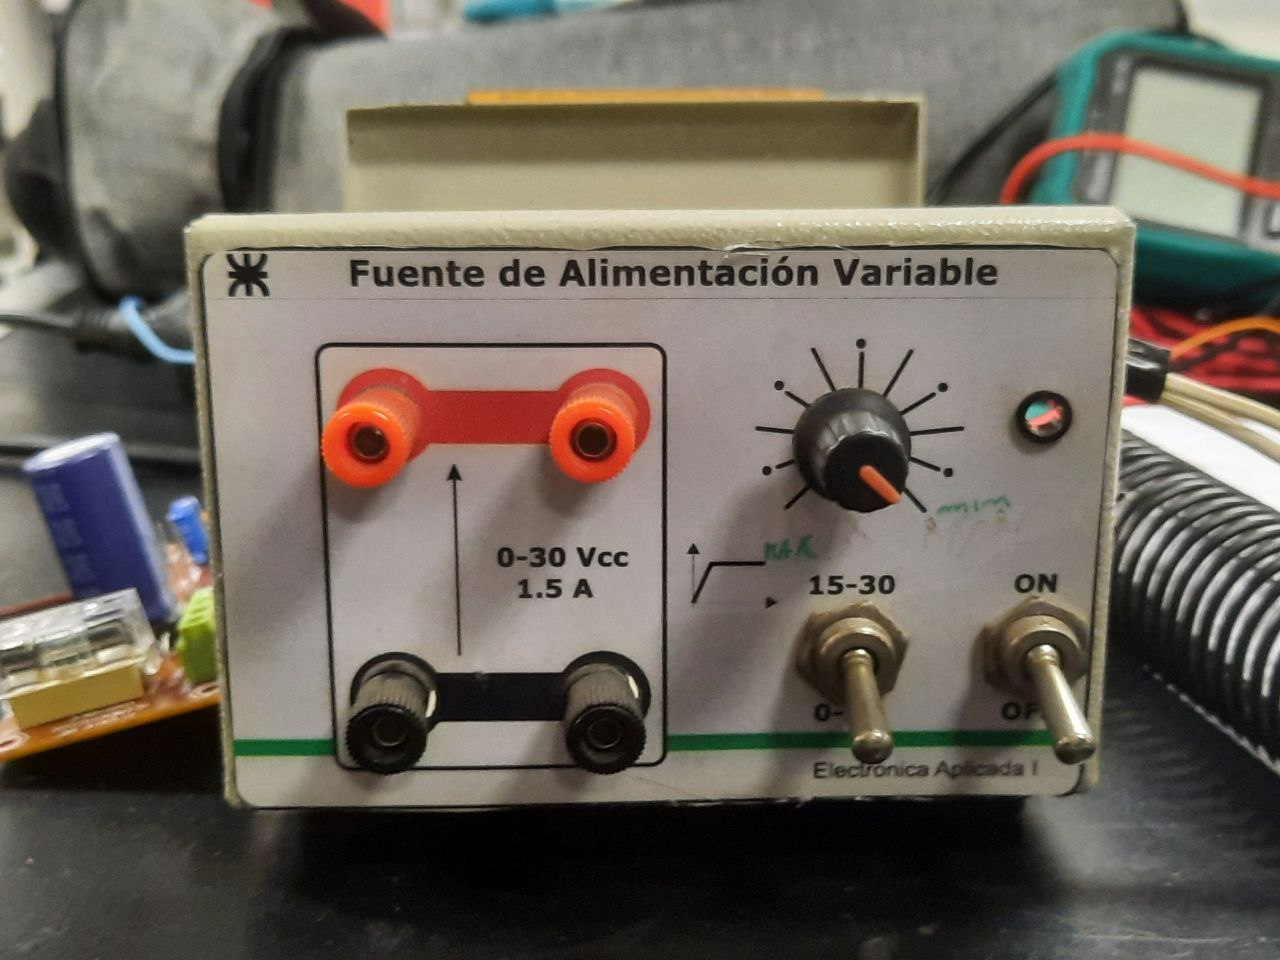
\includegraphics[width=0.9\linewidth]{./imagenes/banco_prueba_frente.jpg}
    \captionof{figure}{Banco de pruebas utilizado en las mediciones.}
\end{center}

\begin{center}
    \centering
    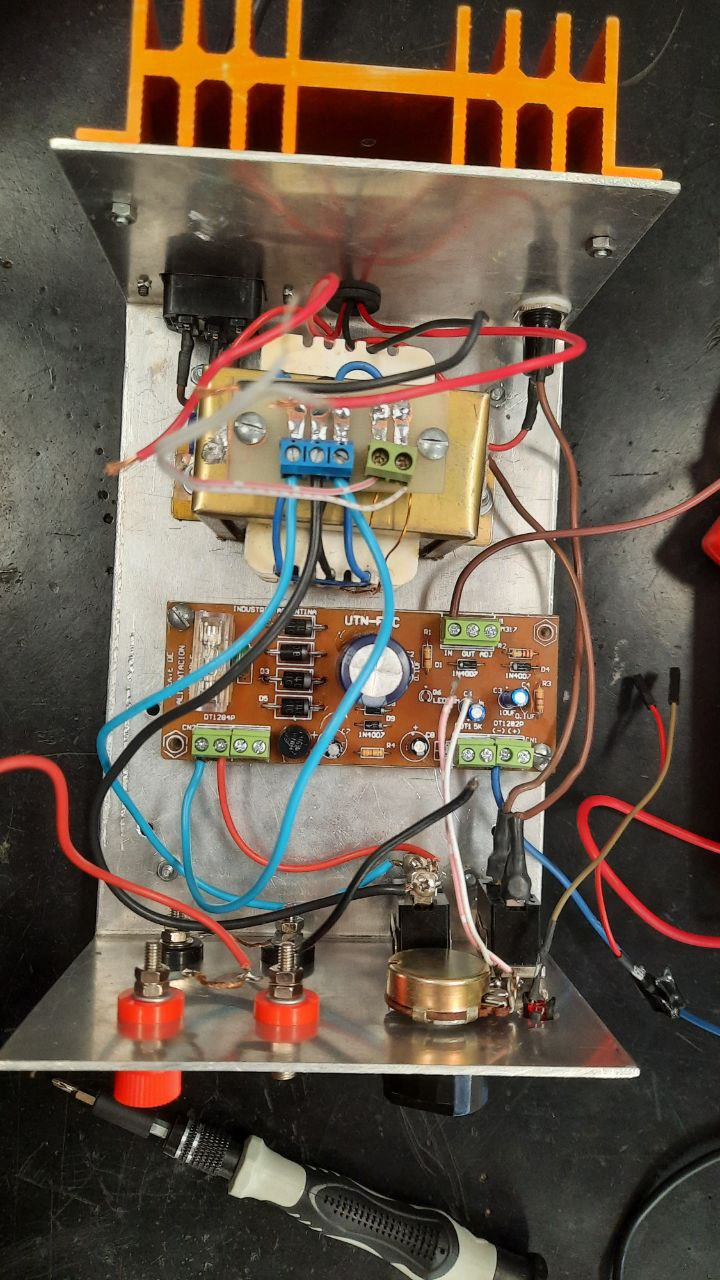
\includegraphics[width=0.9\linewidth]{./imagenes/fuente_completa.jpg}
    \captionof{figure}{Fuente de alimentación ensamblada completamente.}
\end{center}

\begin{center}
    \centering
    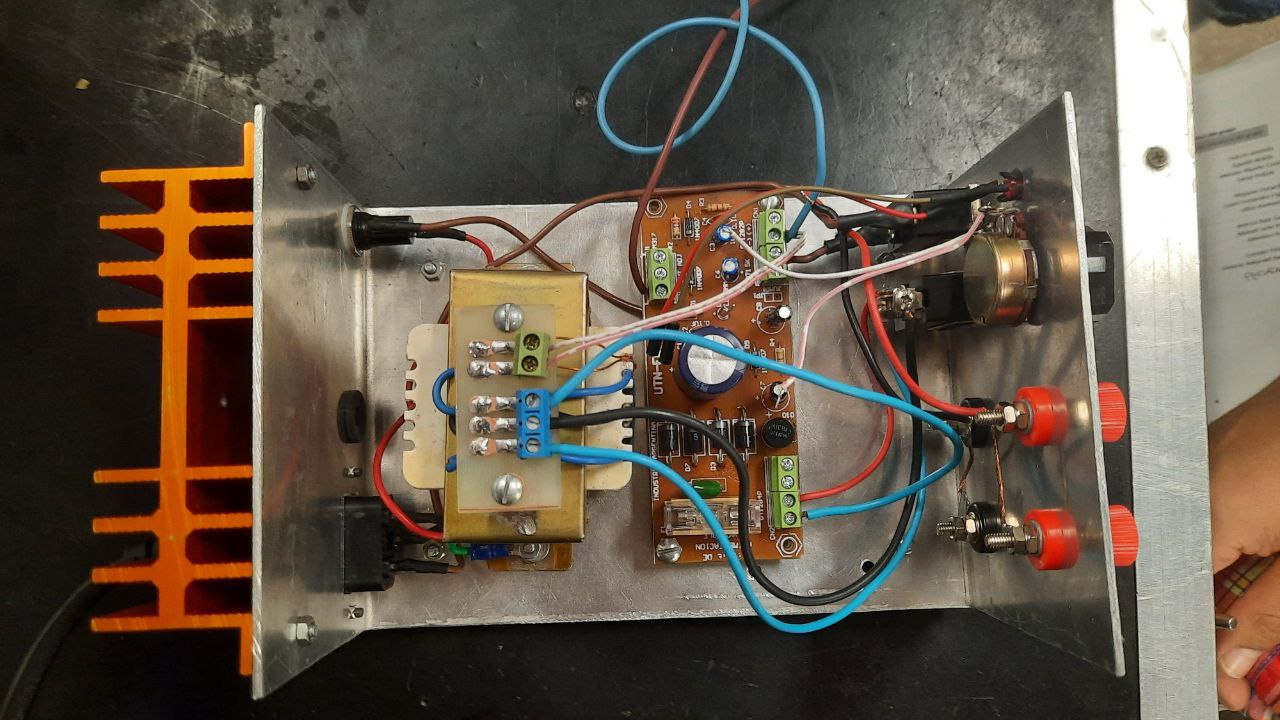
\includegraphics[width=0.9\linewidth]{./imagenes/fuente_sin_LM317.jpg}
    \captionof{figure}{Fuente sin el integrado LM317.}
\end{center}

\begin{center}
    \centering
    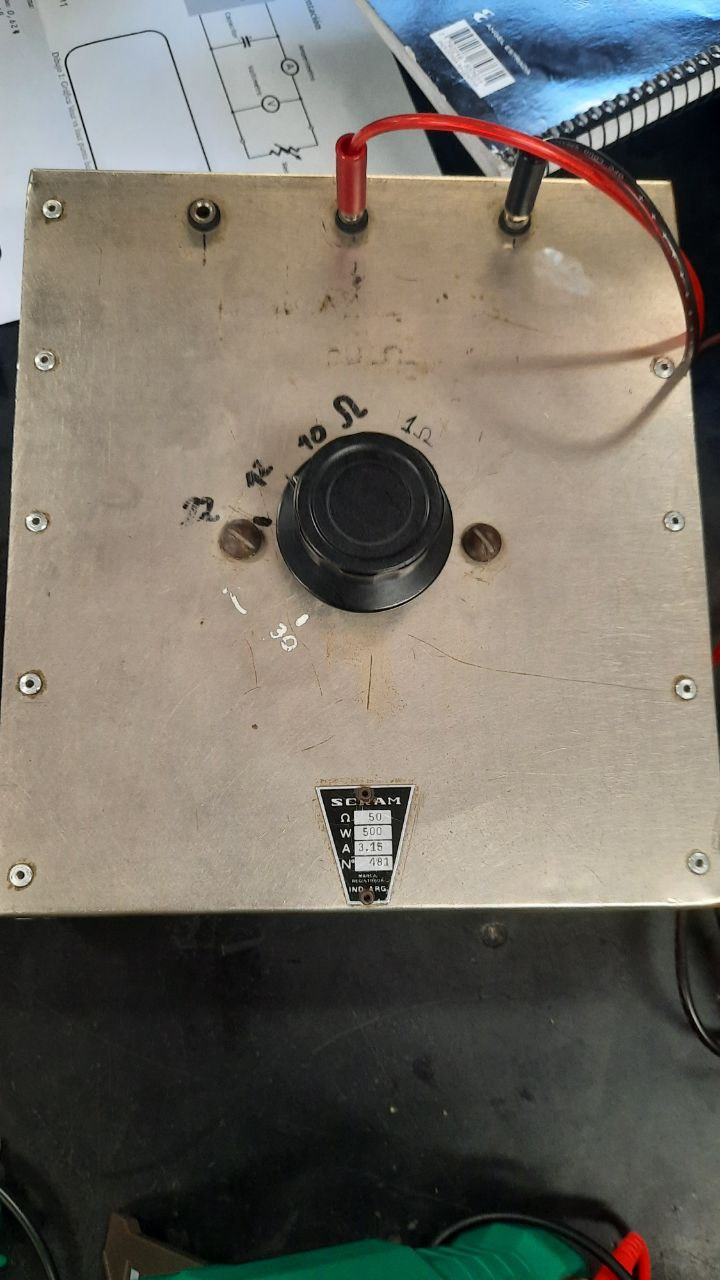
\includegraphics[width=0.9\linewidth]{./imagenes/reostato.jpg}
    \captionof{figure}{Reóstato utilizado en las pruebas.}
\end{center}

\saltoPag{}

% ========== PLACA ==========
\begin{center}
    \centering
    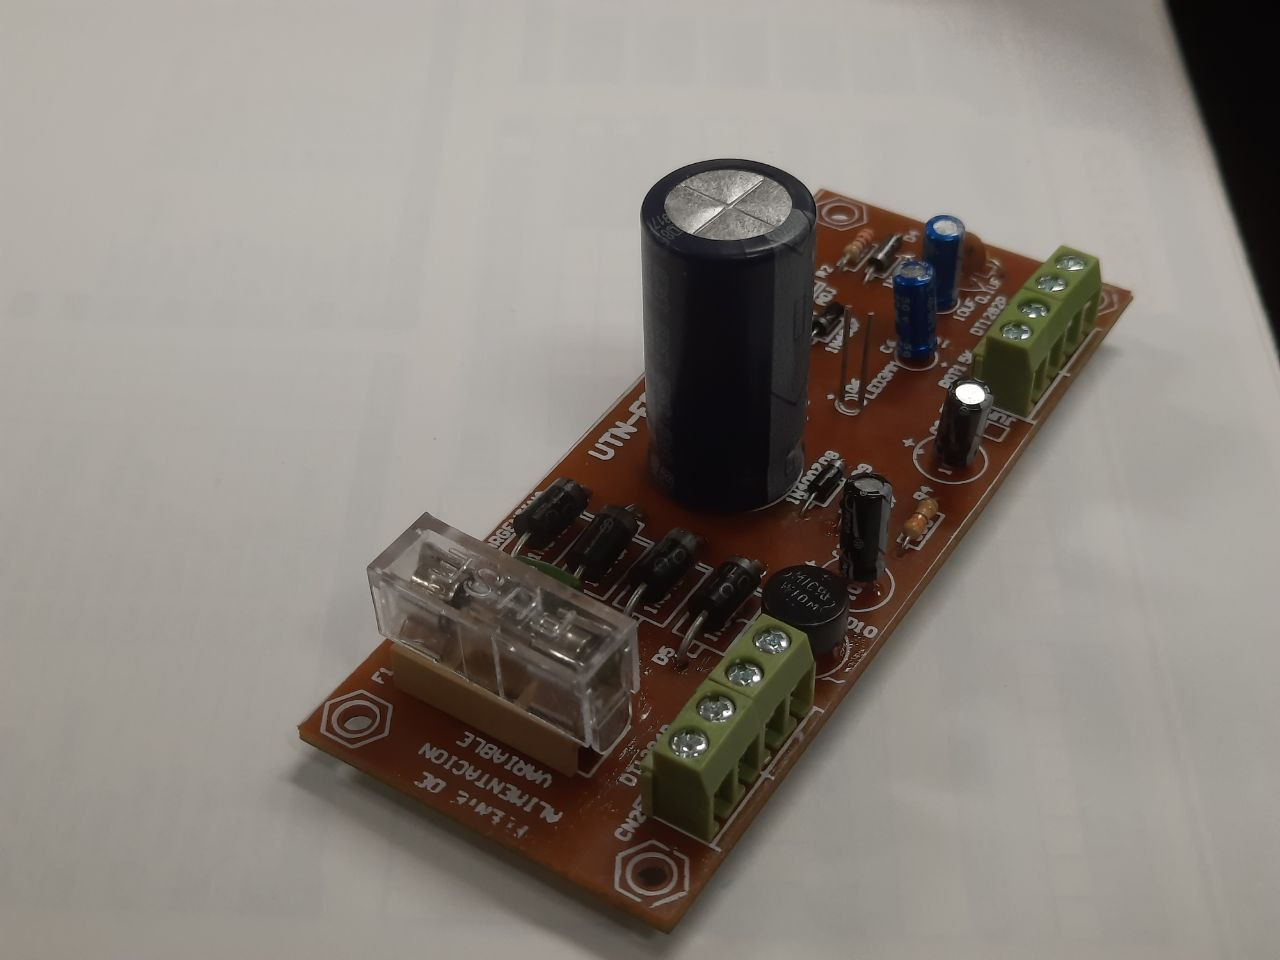
\includegraphics[width=0.9\linewidth]{./imagenes/placa_completa.jpg}
    \captionof{figure}{Placa de circuito impreso terminada.}
\end{center}

% ========== TENSIONES BAJAS ==========

\begin{center}
    \centering
    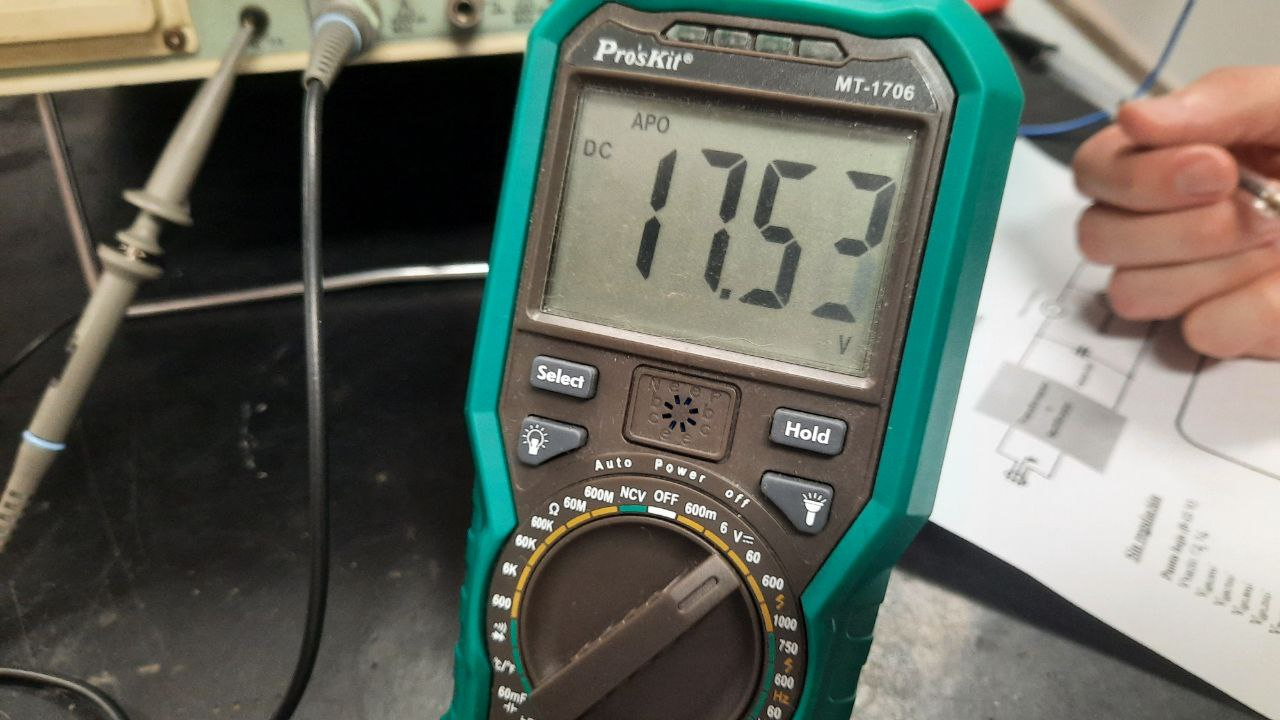
\includegraphics[width=0.9\linewidth]{./imagenes/tension_baja_vacio.jpg}
    \captionof{figure}{Tensión baja en vacío.}
\end{center}


\begin{center}
    \centering
    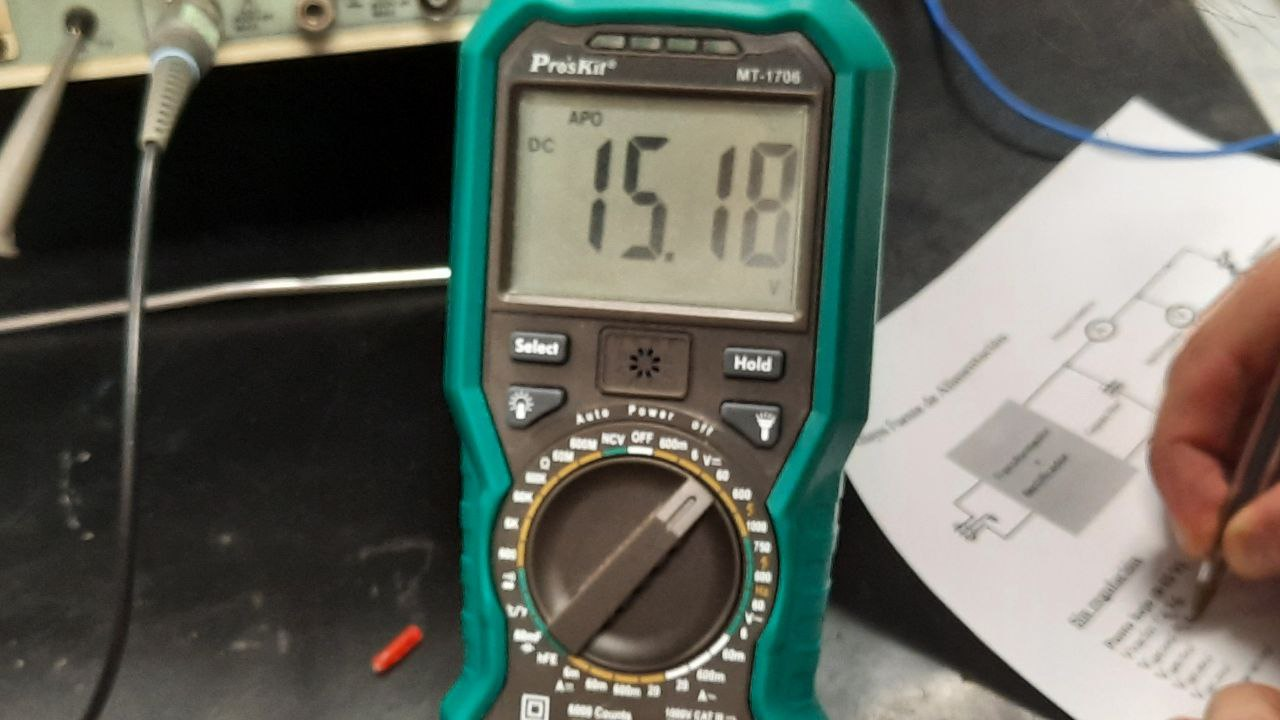
\includegraphics[width=0.9\linewidth]{./imagenes/tension_baja_050.jpg}
    \captionof{figure}{Medición de tensión baja (0.50 V).}
\end{center}

\begin{center}
    \centering
    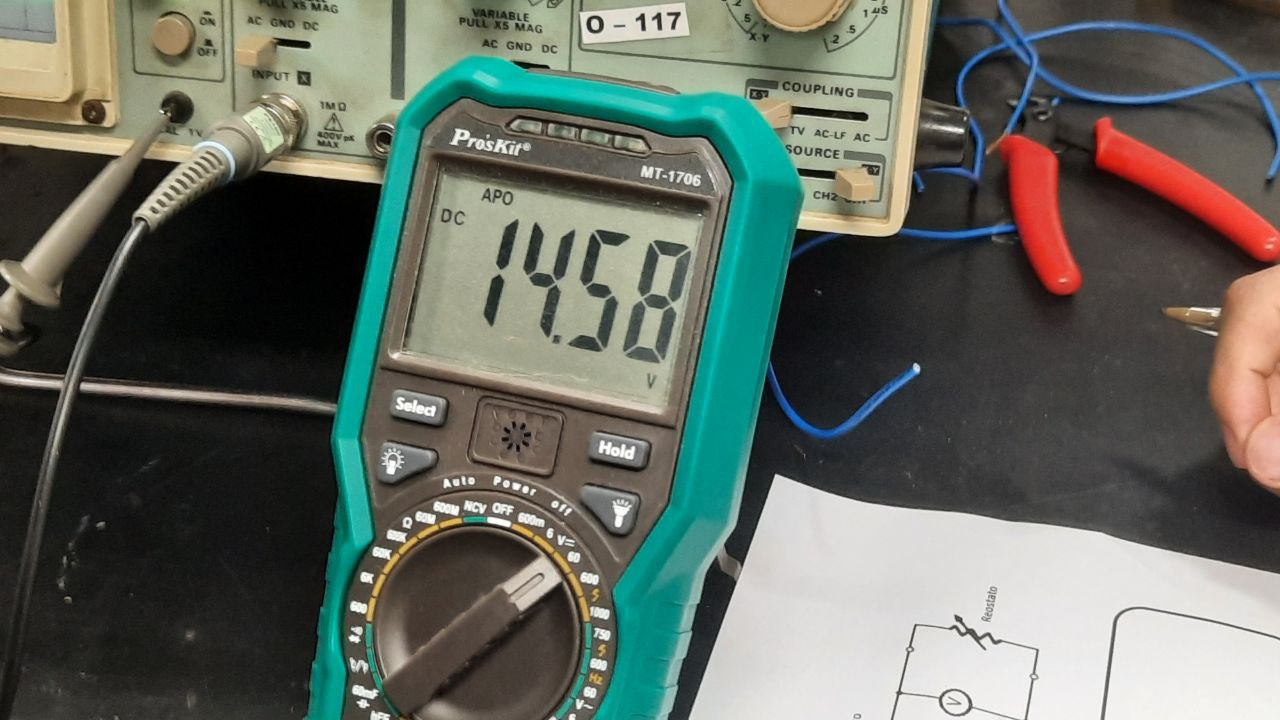
\includegraphics[width=0.9\linewidth]{./imagenes/tension_baja_075.jpg}
    \captionof{figure}{Medición de tensión baja (0.75 V).}
\end{center}

\begin{center}
    \centering
    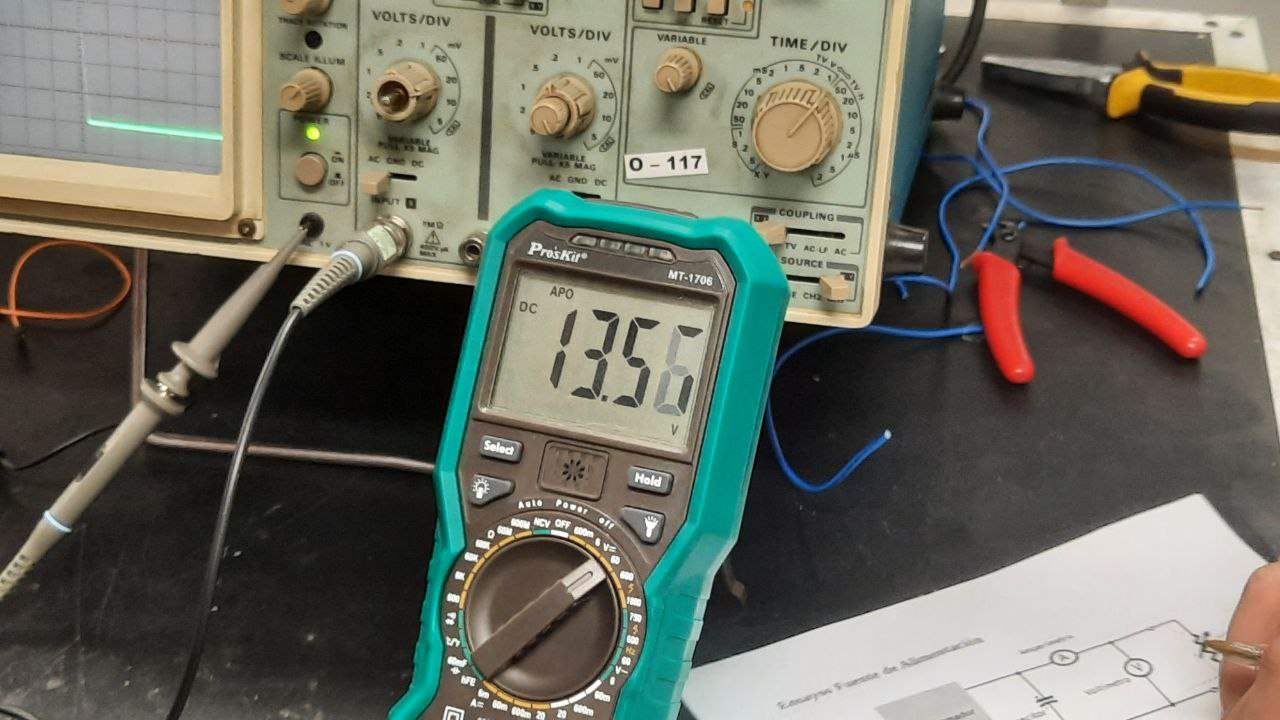
\includegraphics[width=0.9\linewidth]{./imagenes/tension_baja_1,25.jpg}
    \captionof{figure}{Medición de tensión baja (1.25 V).}
\end{center}

\begin{center}
    \centering
    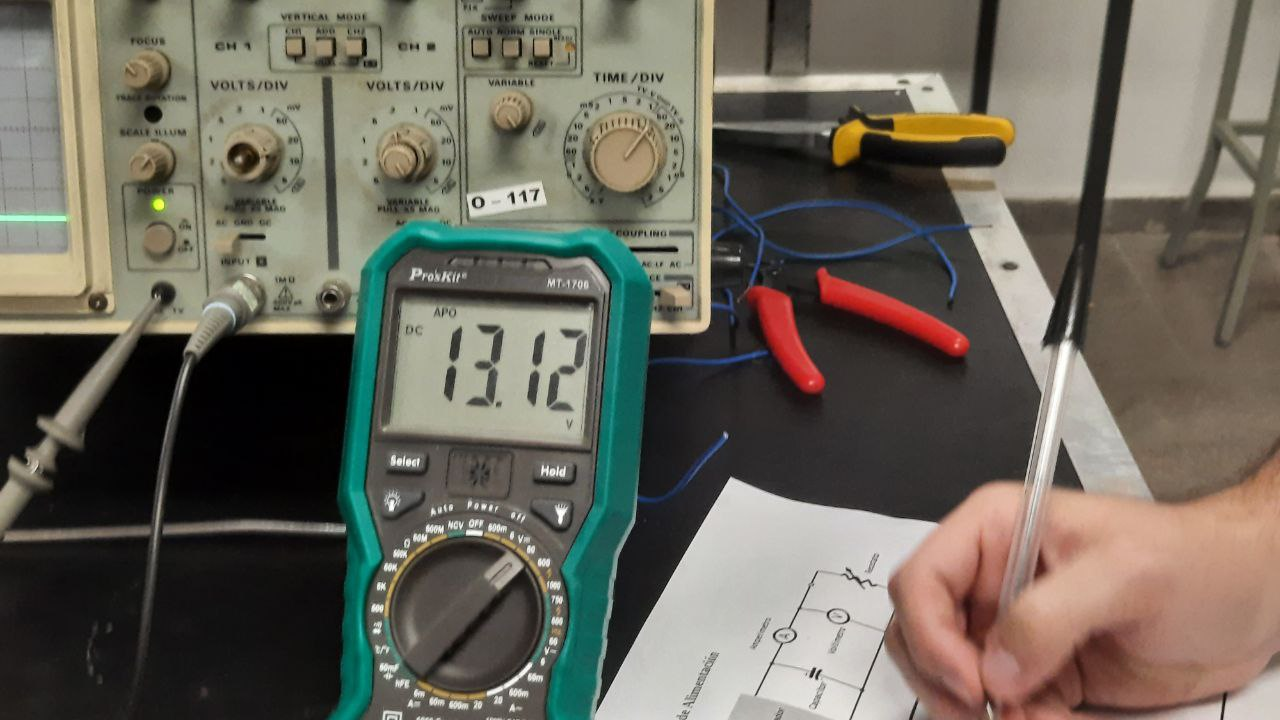
\includegraphics[width=0.9\linewidth]{./imagenes/tension_baja_1,50.jpg}
    \captionof{figure}{Medición de tensión baja (1.50 V).}
\end{center}


% ========== CORRIENTES BAJAS ==========
\begin{center}
    \centering
    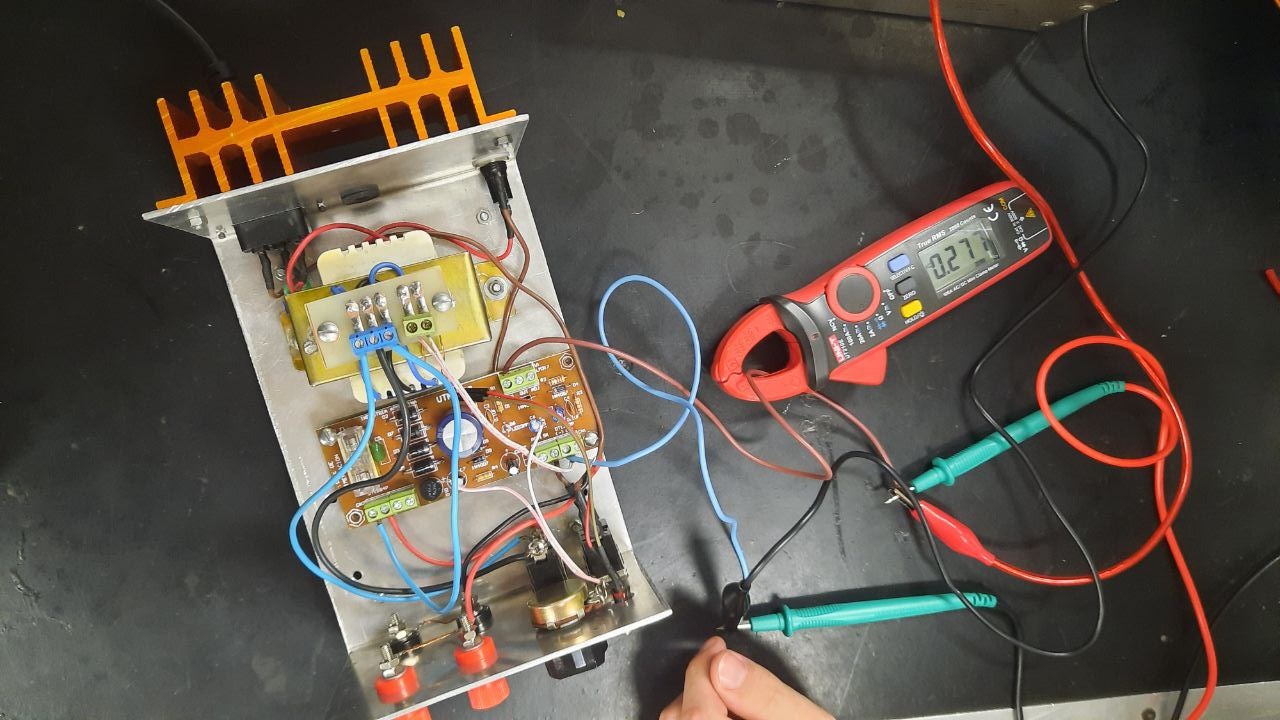
\includegraphics[width=0.9\linewidth]{./imagenes/corriente_baja_0,25.jpg}
    \captionof{figure}{Medición de corriente baja (0.25 A).}
\end{center}

\begin{center}
    \centering
    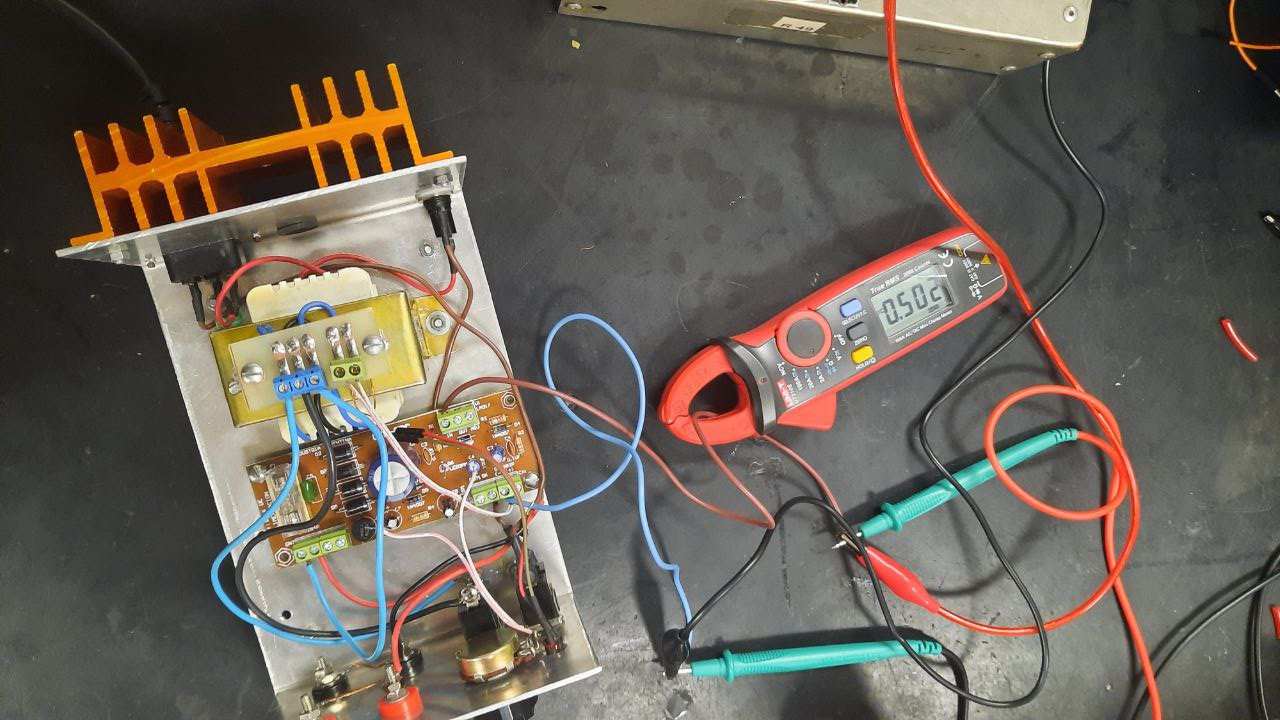
\includegraphics[width=0.9\linewidth]{./imagenes/corriente_baja_050.jpg}
    \captionof{figure}{Medición de corriente baja (0.50 A).}
\end{center}

\begin{center}
    \centering
    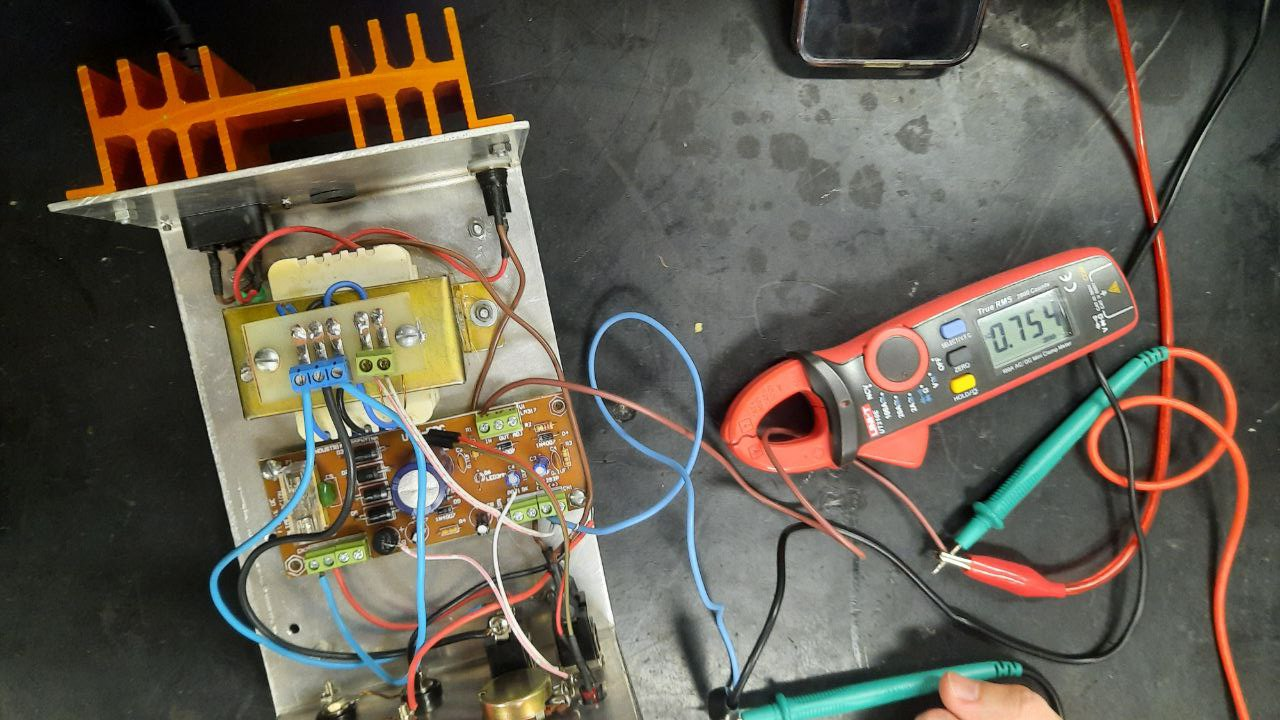
\includegraphics[width=0.9\linewidth]{./imagenes/corriente_baja_075.jpg}
    \captionof{figure}{Medición de corriente baja (0.75 A).}
\end{center}

\saltoPag{}

\begin{center}
    \centering
    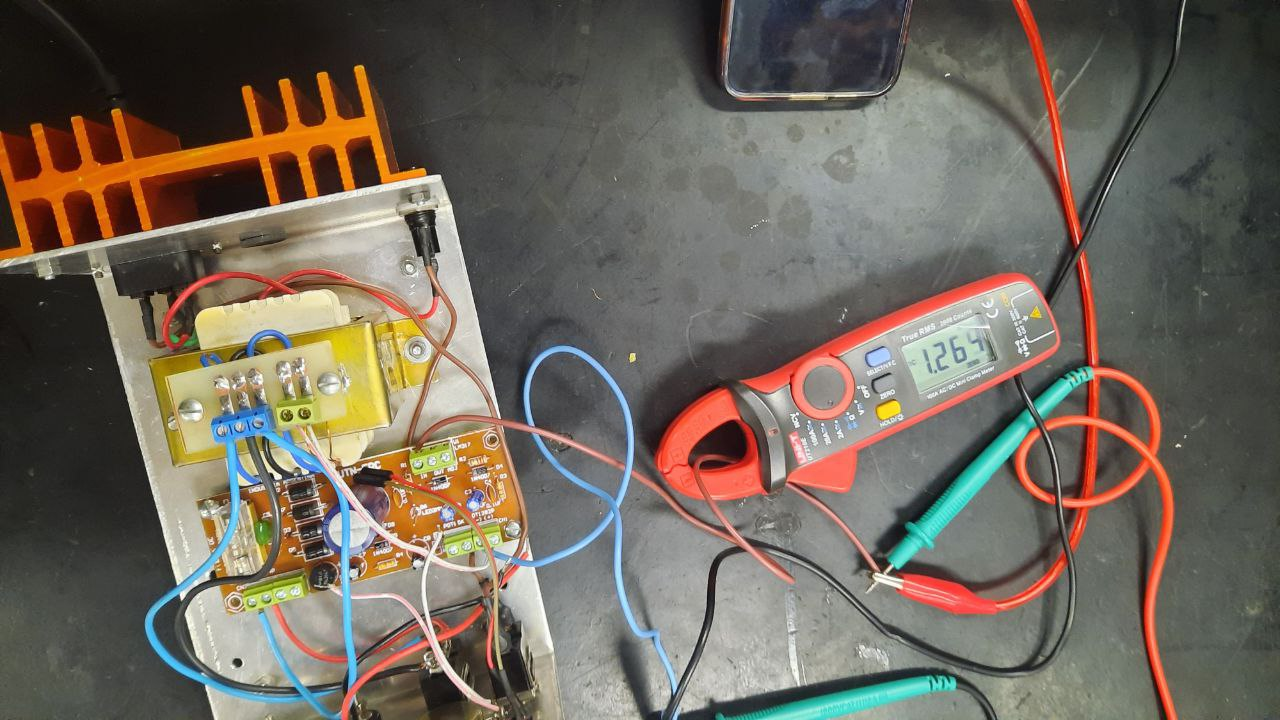
\includegraphics[width=0.9\linewidth]{./imagenes/corriente_baja_1,25.jpg}
    \captionof{figure}{Medición de corriente baja (1.25 A).}
\end{center}

\begin{center}
    \centering
    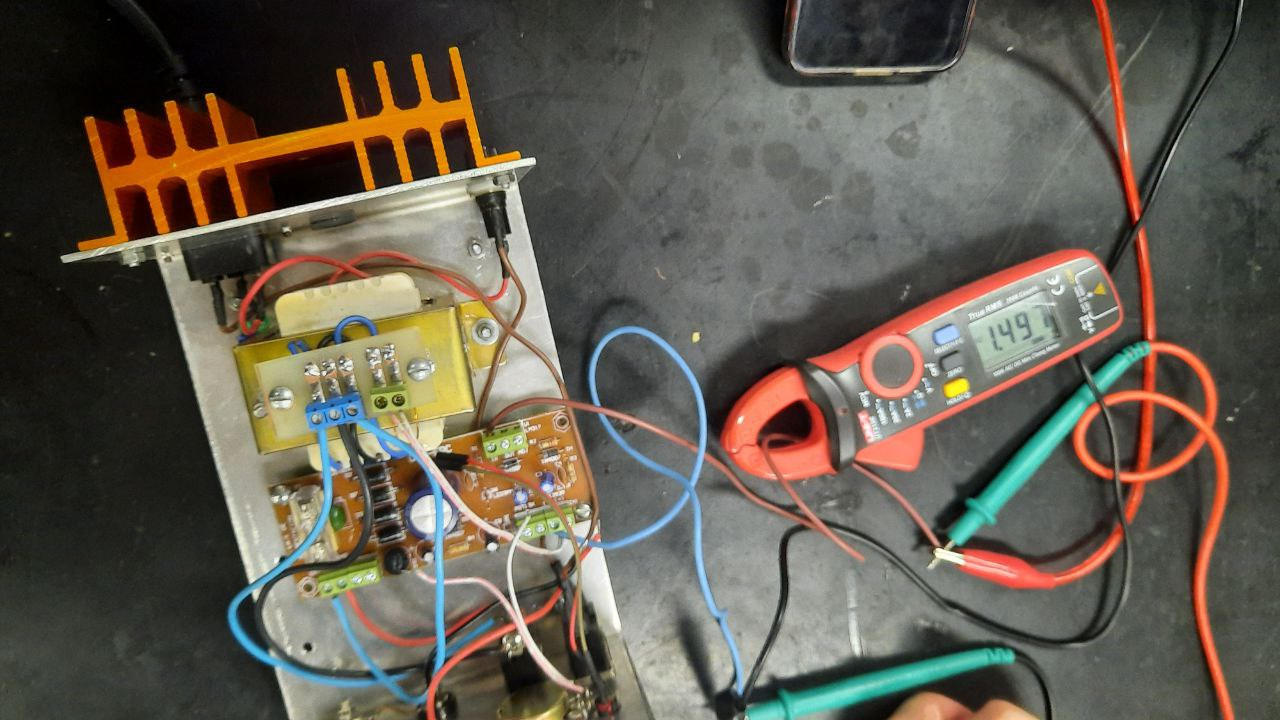
\includegraphics[width=0.9\linewidth]{./imagenes/corriente_baja_1,5.jpg}
    \captionof{figure}{Medición de corriente baja (1.5 A).}
\end{center}

% ========== RIPPLE BAJO ==========
\begin{center}
    \centering
    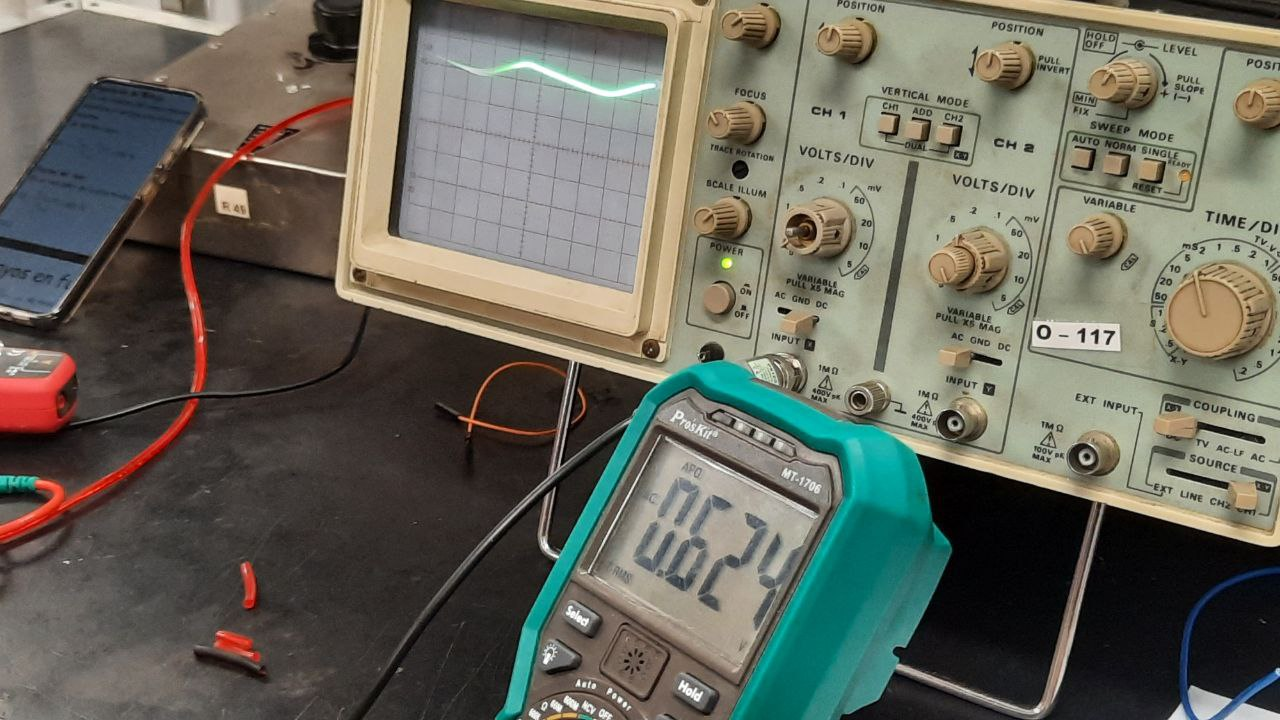
\includegraphics[width=0.9\linewidth]{./imagenes/riplle_baja_osc_mult.jpg}
    \captionof{figure}{Medición de ripple en baja tensión (osciloscopio y multímetro).}
\end{center}

% ========== TENSIONES ALTAS ==========

\begin{center}
    \centering
    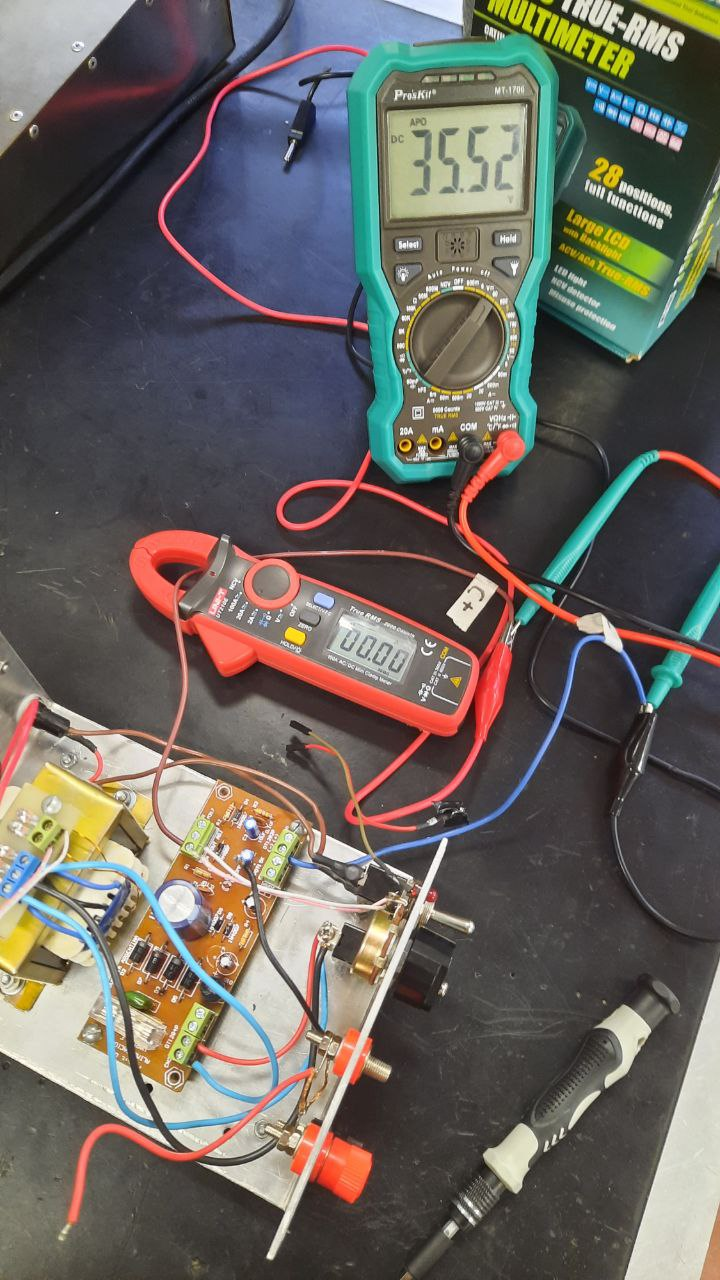
\includegraphics[width=0.9\linewidth]{./imagenes/tension_alta_vacio_rao.jpg}
    \captionof{figure}{Tensión alta en vacío.}
\end{center}


\begin{center}
    \centering
    \includegraphics[width=0.9\linewidth]{./imagenes/tension_alta_0,50.jpg}
    \captionof{figure}{Medición de tensión alta (0.50 V).}
\end{center}

\saltoPag{}

\begin{center}
    \centering
    \includegraphics[width=0.9\linewidth]{./imagenes/tension_alta_0,75.jpg}
    \captionof{figure}{Medición de tensión alta (0.75 V).}
\end{center}

\begin{center}
    \centering
    \includegraphics[width=0.9\linewidth]{./imagenes/tension_alta_1,25.jpg}
    \captionof{figure}{Medición de tensión alta (1.25 V).}
\end{center}

\begin{center}
    \centering
    \includegraphics[width=0.9\linewidth]{./imagenes/tension_alta_1.jpg}
    \captionof{figure}{Medición de tensión alta (1 V).}
\end{center}

\vspace{-0.4cm}

\begin{center}
    \centering
    \includegraphics[width=0.9\linewidth]{./imagenes/tension_alta_1,5.jpg}
    \captionof{figure}{Medición de tensión alta (1.5 V).}
\end{center}

\begin{center}
    \centering
    \includegraphics[width=0.9\linewidth]{./imagenes/temperatura_capsula.jpg}
    \captionof{figure}{Temperatura en la cápsula del componente.}
\end{center}


% ========== CORRIENTES ALTAS ==========
\begin{center}
    \centering
    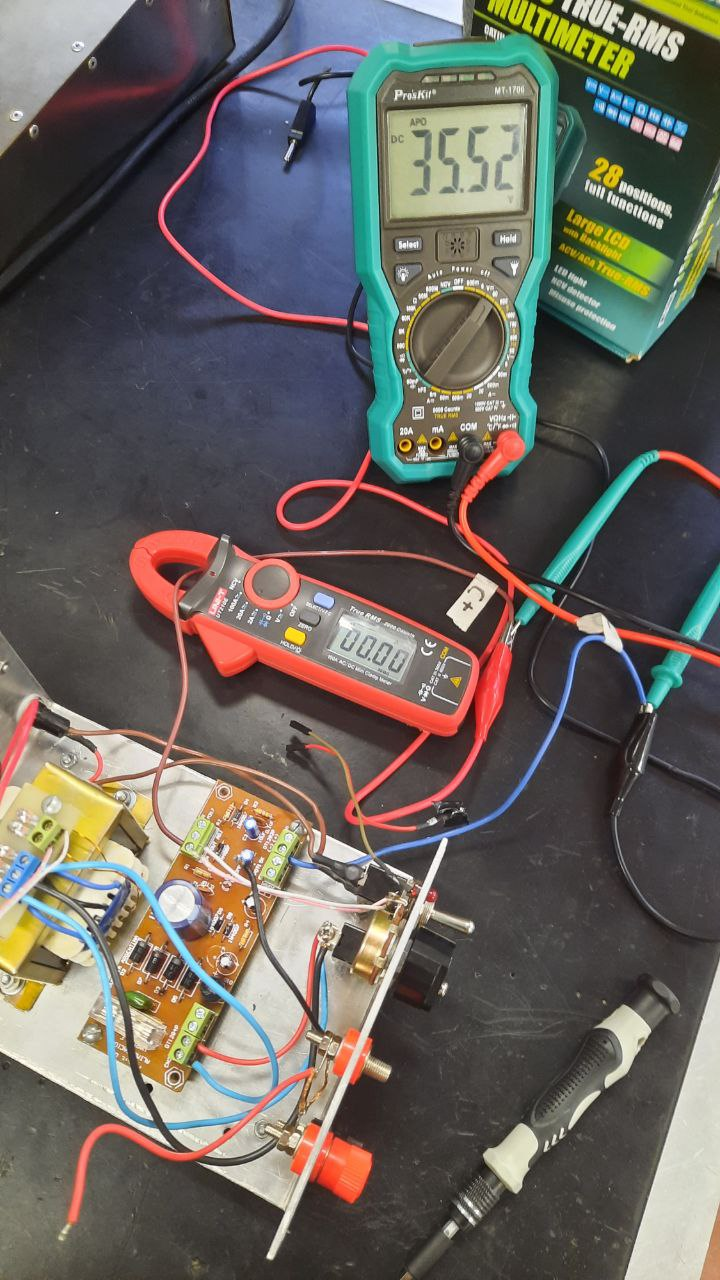
\includegraphics[width=0.9\linewidth]{./imagenes/tension_corriente_alta_vacio.jpg}
    \captionof{figure}{Medición de corriente alta en vacío.}
\end{center}

\saltoPag{}

% ========== RIPPLE ALTO ==========
\begin{center}
    \centering
    \includegraphics[width=0.9\linewidth]{./imagenes/riplle_alta_multimetro.jpg}
    \captionof{figure}{Medición de ripple en alta tensión (multímetro).}
\end{center}

\begin{center}
    \centering
    \includegraphics[width=0.9\linewidth]{./imagenes/riplle_alta_osc.jpg}
    \captionof{figure}{Medición de ripple en alta tensión (osciloscopio).}
\end{center}


\columnbreak{}
\text{}
    \end{multicols}

\end{document}


